\documentclass{beamer-control}
\usepackage{beamer-control-singlefile}
\INCLUDEONLY{Qualitative Analysis}
\begin{document}
\CONCEPT{Qualitative Analysis}

\begin{SUMMARY}
\begin{itemize}
\item Vector fields
\item Phase portraits
\item Equilibrium Points
\item Limit Cycles
\end{itemize}
\vfill References:
\begin{itemize}
\item \astrom{Chapter Z}
\end{itemize}
\end{SUMMARY}



\SUBCONCEPT{Vector fields and Phase portraits}

\begin{frame}
\frametitle{ODE vector field}
Consider the ODE:
\begin{align}
\Deriv{x}{t} = F(x)
\end{align}
\begin{itemize}
\item At every $x$, $F(x)$ defines the `rate of change' of the system
\item We can \emph{plot} this rate of change as a function over state space
\item For a system with two state variables, this is planar plot with a 2D vector defined at all points on the plane
\item This plot is known as a \emph{vector field plot}, or \emph{quiver} plot (\texttt{quiver()} in Matlab)
\end{itemize}
\end{frame}

\begin{frame}
\frametitle{ODE vector field plot}
\framesubtitle{Note the positions of zero vector}
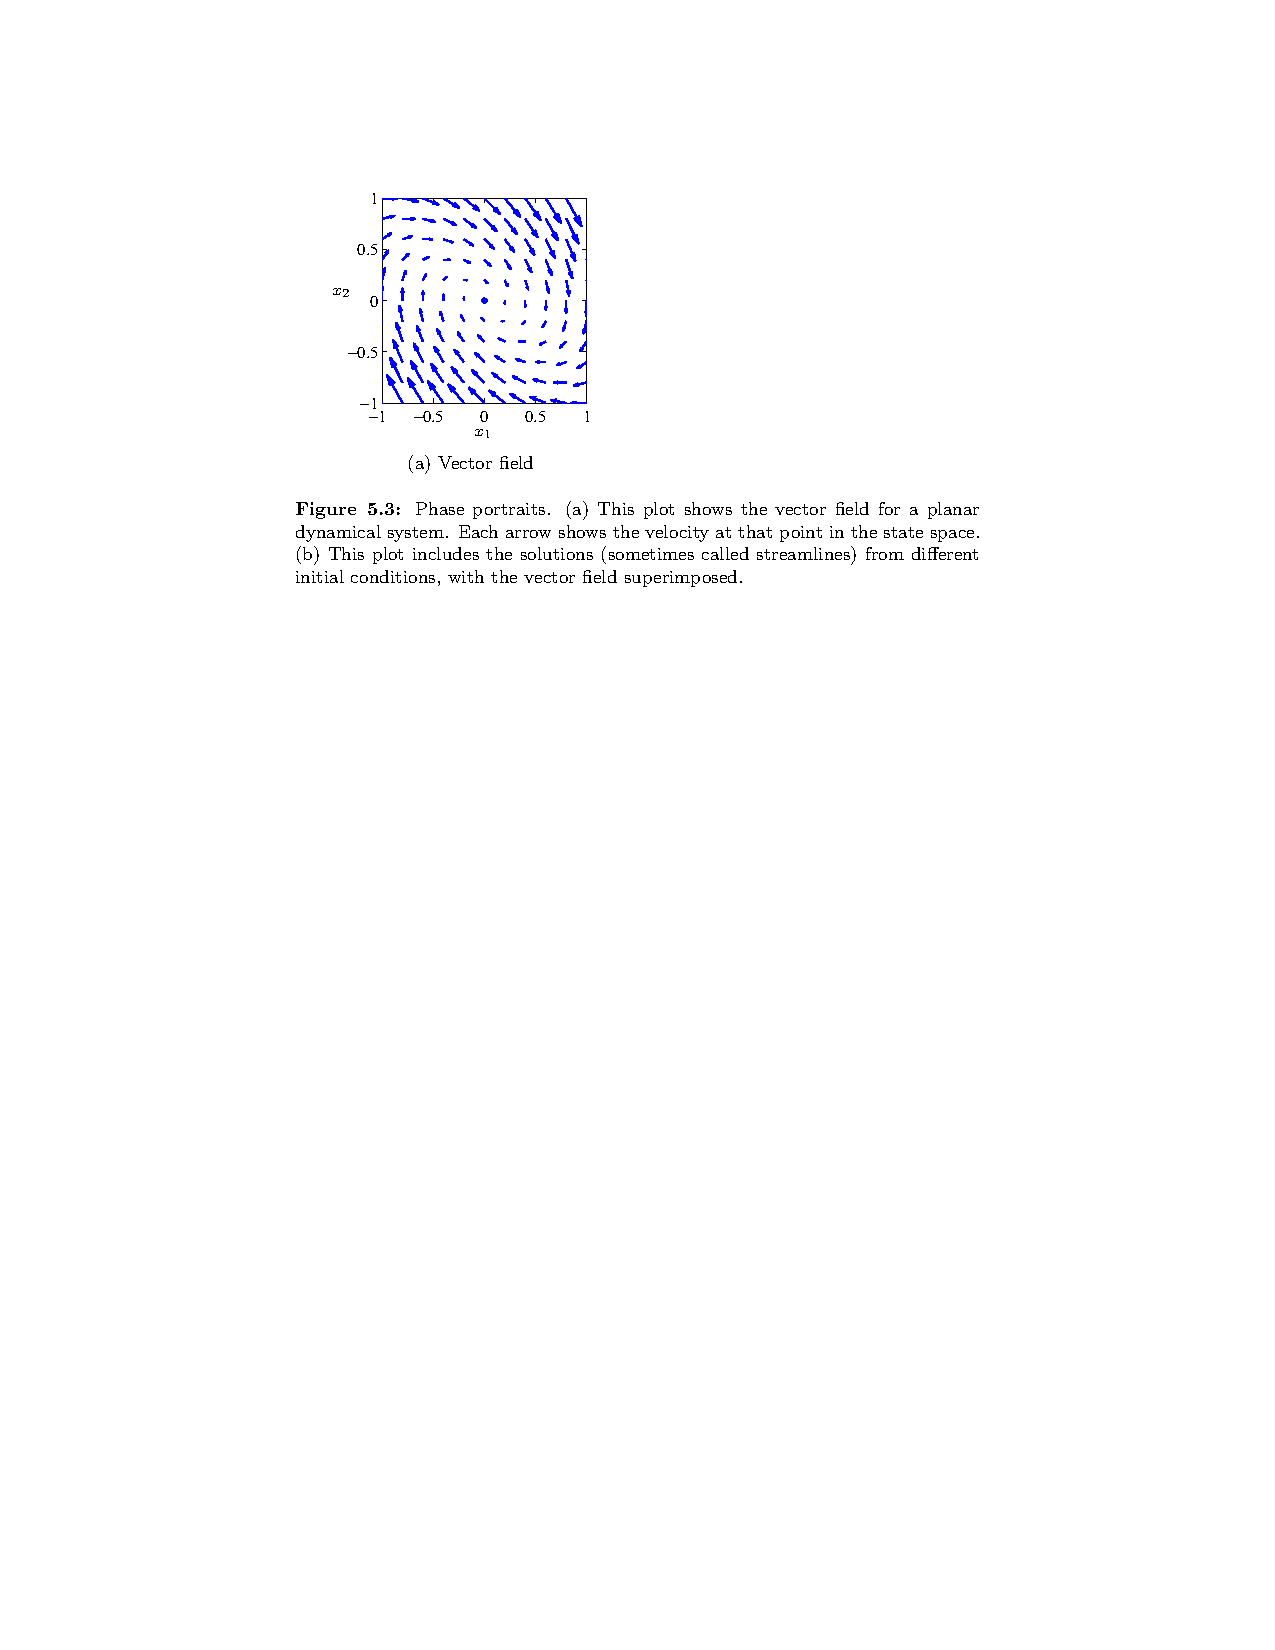
\includegraphics[width=\linewidth]{figure5.3a}
\end{frame}

\begin{frame}
\frametitle{Phase portrait}
\begin{itemize}
\item The vector field is best at highlighting stationary points
\item You can infer but can't directly visualise trajectories
\item Enter the `phase portrait' --- a superimposed collection of trajectories 
\item Where the trajectories cluster and converge tells us important properties of the system
\item Note that trajectories don't tell us rate of change
\end{itemize}
\end{frame}

\begin{frame}
\frametitle{Phase portrait plot}
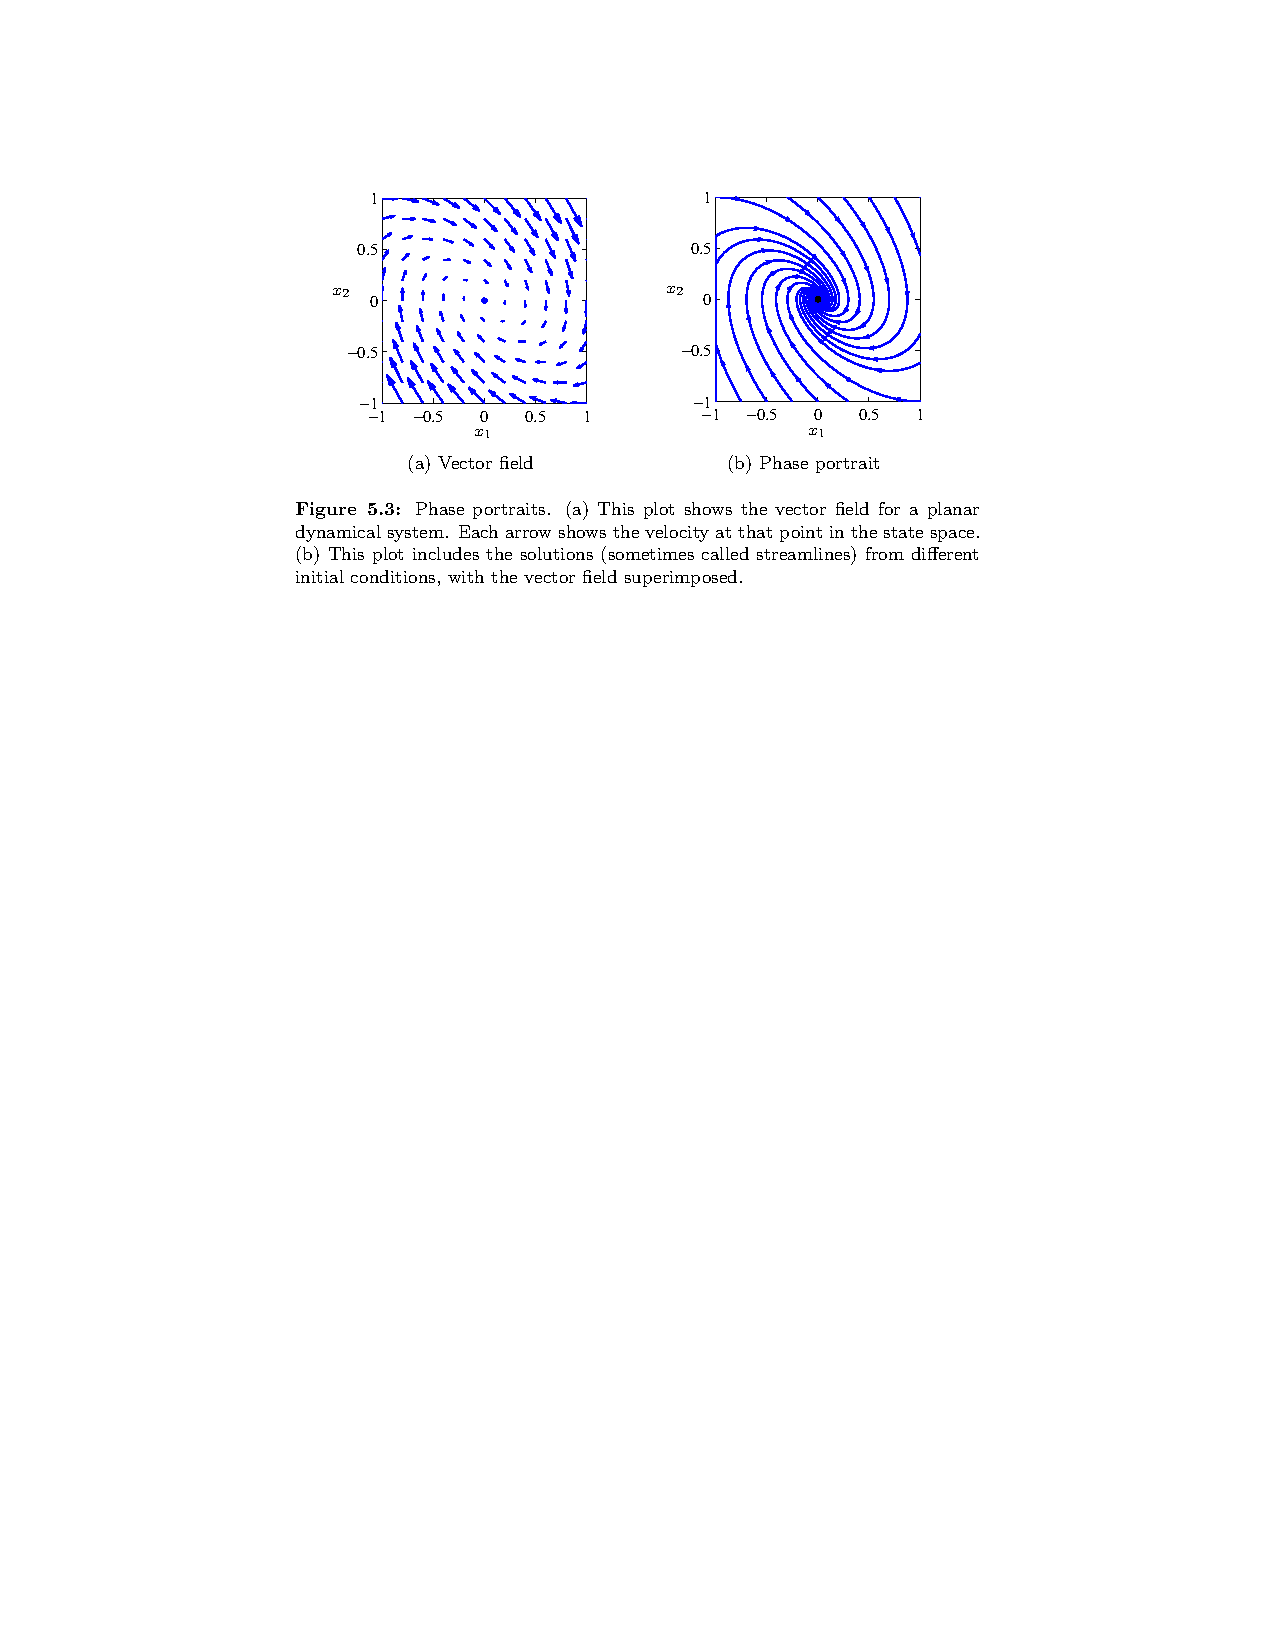
\includegraphics[width=\linewidth]{figure5.3b}

\end{frame}

\SUBCONCEPT{Equilibrium Points and Limit Cycles}

\begin{frame}{This is another slide}
\begin{itemize}
\item c
\item d
\end{itemize}
\end{frame}


\SUMMARYFRAME
\FINALE

\end{document}
